\chapter{Quan hệ hai ngôi}

\section{Quan hệ hai ngôi}

\begin{definition}[Quan hệ hai ngôi]
    Xét hai tập hợp $A$ và $B$. Ta gọi $\mathcal{R}$ là một quan hệ hai ngôi trên $A$ và $B$ nếu $\mathcal{R} \subset A \times B$. Trong đó $A \times B$ là tích Descartes của hai tập hợp.
\end{definition}

Nếu phần tử $(a, b) \in R$ với $a \in A$ và $b \in B$ thì ta nói \textbf{$a$ có quan hệ với $b$} và ký hiệu $a \mathcal{R} b$.

Khi $A \equiv B$ thì ta nói $\mathcal{R}$ là quan hệ hai ngôi trên $A$. Đây cũng là yếu tố quan trọng cho các khái niệm về sau.

\begin{example}
    Xét hai tập hợp $A = \{1, 2, 3, 4\}$ và $B = \{a, b, c\}$. Khi đó tích Descartes 
    \begin{align*}
        A \times B = \{
        & (1, a), (1, b), (1, c), (2, a), (2, b), (2, c), \\
        & (3, a), (3, b), (3, c), (4, a), (4, b), (4, c)
    \}
    \end{align*}

    Giả sử $\mathcal{R} = \{(1, a), (3, b), (4, c)\}$ thì 1 quan hệ với $a$ do $(1, a) \in \mathcal{R}$, hay $1 R a$. Tuy nhiên 1 không có quan hệ với $b$ do $(1, b) \not\in \mathcal{R}$.
\end{example}

Sau đây ta định nghĩa các loại quan hệ hai ngôi.

\begin{definition}
    Cho $R$ là quan hệ hai ngôi trên tập $A$. Ta nói
    \begin{enumerate}
        \item $\mathcal{R}$ \textbf{phản xạ} (hay \textbf{reflexive}) nếu với mọi $x \in A$ thì $(x, x) \in \mathcal{R}$;
        \item $\mathcal{R}$ \textbf{đối xứng} (hay \textbf{symmetric}) nếu $(x, y) \in \mathcal{R}$ thì $(y, x) \in \mathcal{R}$;
        \item $\mathcal{R}$ \textbf{phản xứng} (hay \textbf{antisymmetric}) nếu $(x, y) \in \mathcal{R}$ thì $(y, x) \not\in \mathcal{R}$. Nói cách khác nếu $(x, y) \in \mathcal{R}$ và $(y, x) \in \mathcal{R}$ thì $x = y$;
        \item $\mathcal{R}$ \textbf{bắc cầu} (hay \textbf{transitive}) nếu $(x, y) \in \mathcal{R}$ và $(y, z) \in \mathcal{R}$ thì $(x, z) \in \mathcal{R}$.
    \end{enumerate}
\end{definition}

\subsection*{Quan hệ tương đương}

Quan hệ tương đương giúp ta chia (phân hoạch) một tập hợp rời rạc thành các tập con mà chỉ cần một phần tử đại diện cho tập con đó là đủ để tính toán.

\begin{definition}[Quan hệ tương đương]
    Cho $\mathcal{R}$ là quan hệ trên tập $A$. Khi đó $\mathcal{R}$ được gọi là \textbf{quan hệ tương đương} nếu $\mathcal{R}$ phản xạ, đối xứng và bắc cầu.

    Ta có thể ký hiệu $x \mathcal{R} y$ với $\mathcal{R}$ là quan hệ tương đương là $x \sim y$ hoặc $x \widetilde{\mathcal{R}} y$.
\end{definition}

Tiếp theo ta định nghĩa lớp tương đương chứa phần tử $x$ và tập thương.

\begin{definition}[Lớp tương đương]
    Cho $\mathcal{R}$ là quan hệ tương đương trên tập $A$. Khi đó với $x \in A$, ta định nghĩa lớp tương đương chứa phần tử $x$ là tập các phần tử của $A$ có quan hệ với $x$ \[ \bar{x} = \{ y \in A, \, y \mathcal{R} x \} \]
\end{definition}

\begin{definition}[Tập thương]
    Tập hợp các lớp tương đương như trên tạo thành tập thương.
    \[A / \mathcal{R} = \{ \bar{x}, \, x \in A \}\]
\end{definition}

\begin{example}
    Xét số nguyên dương $n$. Với số nguyên $x$ và $y$, ta nói $x$ có quan hệ với $y$ nếu $n \vert (x - y)$, hay $x \equiv y \bmod n$. Ta ký hiệu quan hệ này là $n \ZZ$.

    Quan hệ trên là quan hệ tương đương vì
    \begin{enumerate}
        \item $n \vert 0 = x - x$ với mọi $x \in \ZZ$ nên có tính phản xạ;
        \item $n \vert (x - y) \Rightarrow n \vert -(x-y) = y-x$  với mọi $x, y \in \ZZ$ nên có tính đối xứng;
        \item $n \vert (x - y)$ và $n \vert (y - z)$ thì $n \vert (x - y + y - z) = (x - z)$ nên có tính bắc cầu.
    \end{enumerate}

    Từ đó ta có thể phân tập $\ZZ$ thành các lớp tương đương
    \begin{align*}
        \overline{0} & = \{ \ldots, -2n, -n, 0, n, 2n, \ldots \} \\
        \overline{1} & = \{ \ldots, -2n+1, -n+1, 1, n+1, 2n+1, \ldots \} \\
        \vdots \\
        \overline{n-1} & = \{ \ldots, -n-1, -1, n-1, 2n-1, 3n-1, \ldots \}
    \end{align*}

    Tập thương của chúng ta là $\ZZ / n\ZZ = \{ \overline{0}, \overline{1}, \ldots, \overline{n-1} \}$.
\end{example}

\subsection*{Quan hệ thứ tự}

\begin{definition}[Quan hệ thứ tự]
    Cho quan hệ $\mathcal{R}$ trên tập $A$. Ta nói $\mathcal{R}$ là quan hệ thứ tự nếu $\mathcal{R}$ phản xạ,  phản xứng và bắc cầu.
\end{definition}

\begin{definition}
    Cho tập hợp $A$ và quan hệ $\mathcal{R}$ trên $A$ là quan hệ thứ tự. Nếu $x \mathcal{R} y$ thì ta ký hiệu $x \prec y$. Khi đó $(A, \prec)$ được gọi là \textbf{tập có  thứ tự}.
\end{definition}

Tiếp theo là một số định nghĩa quan trọng về tập hợp có thứ tự.

\begin{definition}
    Với $(A, \prec)$ và $x, y \in A$,
    \begin{enumerate}
        \item Nếu $x \prec y$, ta nói \textbf{$y$ là trội của $x$}, hay là \textbf{$x$ được trội bởi $y$};
        \item $y$ là \textbf{trội trực tiếp} của $x$ nếu không tồn tại $z$ sao cho $x \prec z$ và $z \prec y$.
    \end{enumerate}
\end{definition}

\begin{definition}
    Xét $(A, \prec)$.
    \begin{enumerate}
        \item $x$ và $y$ thuộc $A$ được gọi là \textbf{so sánh được} nếu $x \prec y$ hoặc $y \prec x$;
        \item nếu với mọi $x, y \in A$, $x$ và $y$ so sánh được thì $(A, \prec)$ được gọi là \textbf{quan hệ thứ tự toàn phần}. Ngược lại thì gọi là \textbf{quan hệ thứ tự bán phần}.
    \end{enumerate}
\end{definition}

Để biểu diễn sự so sánh trong một tập hợp, ta sử dụng biểu đồ Hasse.

\begin{definition}
    Biểu đồ Hasse của $(A, \prec)$ với $A$ là tập hữu hạn bao gồm
    \begin{enumerate}
        \item Tập điểm - mỗi điểm biểu diễn một phần tử của $A$;
        \item Tập cung - vẽ một cung từ $x$ tới $y$ nếu $y$ là trội trực tiếp của $x$.
    \end{enumerate}
\end{definition}

\begin{example}
    Xét tập $U_{12} = \{ 1, 2, 3, 4, 6, 12 \}$ với quan hệ $x \mathcal{R} y$ được định nghĩa $x$ là ước của $y$.

    Theo đó, biểu đồ Hasse của quan hệ trên là hình \ref{hasse:1}.
    \begin{figure}[ht]
        \centering
        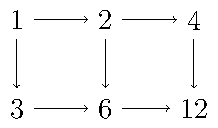
\includegraphics{figures/hasse/hasse1.pdf}
        \caption{Biểu đồ Hasse của $U_{12}$}
        \label{hasse:1}
    \end{figure}
\end{example}

\begin{definition}
    Xét quan hệ thứ tự $(A, \prec)$.
    \begin{enumerate}
        \item Phần tử $M \in A$ được gọi là
        \begin{enumerate}
            \item \textbf{Tối đại} nếu $M \prec x$ thì $x = M$;
            \item \textbf{Cực đại} (hay \textbf{lớn nhất}) nếu với mọi $x \in A$ thì $x \prec M$.
        \end{enumerate}
        \item Phần tử $m \in A$ được gọi là
        \begin{enumerate}
            \item \textbf{Tối tiểu} nếu $x \prec m$ thì $x = m$;
            \item \textbf{Cực tiểu} (hay \textbf{nhỏ nhất}) nếu với mọi $x \in A$ thì $m \prec x$.
        \end{enumerate}
    \end{enumerate}
\end{definition}

\begin{remark}
    \begin{enumerate}
        \item Phần tử cực đại nếu có là duy nhất. Tương tự cho cực tiểu;
        \item Nếu $n$ là phần tử tối đại duy nhất thì nó cũng là cực đại. Tương tự cho tối tiểu.
    \end{enumerate}
\end{remark}

Trong ví dụ $U_{12}$ ở trên thì 1 là tối tiểu và cũng là cực tiểu, và 12 là tối đại và cũng là cực đại.
